% =============================================================
% REVISED MANUSCRIPT v2 -- FRAMEWORK PAPER
% Target: IEEE Transactions on Robotics, regular paper, initial
% submission (12 pages max incl. references; abstract <= 200 words and
% <= 1200 characters in PaperCept; double-anonymous review).
%
% Scope decisions (2026-10-25):
%   * Contact vs. no-contact modelling is the subject of a companion
%     paper and is NOT compared here. The wall-aware model is used as
%     one module of the framework.
%   * U-shape path dropped.
%   * Null-space posture term disabled (gamma = 0) in every hardware run.
%   * Code will not be released; Algorithm 1 and the parameter tables
%     must therefore be complete enough to reimplement the framework.
%
% Markers:
%   \TBD{..}     value that exists in your data/logs but is not in the
%                draft yet (red).
%   \NEWRUN{..}  result of an experiment or analysis that has NOT been
%                run yet (blue). The text around it is written for the
%                planned experiment; it must be replaced by what the run
%                actually shows, including if the outcome differs.
%   % AUTHOR CHECK:  inference the authors must confirm.
%   \figph{..}   figure placeholder at final size.
% =============================================================
\documentclass[journal]{IEEEtran}

\usepackage{amsmath,amssymb,amsfonts}
\usepackage{graphicx}
\usepackage{booktabs}
\usepackage{array}
\usepackage{xcolor}
\usepackage{cite}
\usepackage{algorithm}
\usepackage{algpseudocode}
\usepackage{tikz}
\usetikzlibrary{arrows.meta,positioning,calc,fit,backgrounds,decorations.pathreplacing}

\newcommand{\TBD}[1]{\textcolor{red}{[#1]}}
\newcommand{\NEWRUN}[1]{\textcolor{blue}{[#1]}}
\newcommand{\figph}[3]{%
  \fbox{\parbox[c][#2][c]{\dimexpr#1-2\fboxsep-2\fboxrule\relax}{%
  \centering\footnotesize\textcolor{gray}{\textbf{Figure placeholder}}\\[2pt]
  \parbox{0.9\linewidth}{\centering\footnotesize\textcolor{gray}{#3}}}}}

\begin{document}

\title{An Offline--Online Framework for Real-Time, Constraint-Aware
Predictive Navigation of Magnetic Continuum Robots With a Robot-Mounted
Permanent Magnet}

\author{Anonymous Authors%
\thanks{Manuscript submitted for review to IEEE Transactions on Robotics.}}

\markboth{IEEE Transactions on Robotics}{Offline--Online Predictive
Navigation of Magnetic Continuum Robots}

\maketitle

% Timing (A1, 26 Oct): the loop sleeps a full period after each solve, so
% the realized period is dt + solve time (125.3 ms at N=15 on the vessel).
% The abstract therefore claims the solve fits the 100 ms period, not a
% realized 10 Hz. Switch to fixed-rate scheduling before new runs.
\begin{abstract}
Steering a magnetic continuum robot (MCR) with a robot-mounted permanent
magnet couples a nonuniform field to the arm's joints and delay, near
the patient. Existing controllers trade model fidelity for speed and rarely enforce
safety inside the optimizer. We present a framework that carries a Cosserat model through to
real-time joint commands.
Offline, it solves a configuration at every path node, time-parameterizes
the path under actuator limits, and precomputes a Jacobian schedule by
implicit differentiation, at 0.45--6\,s per Jacobian. Online, a
delay-aware model predictive controller uses the schedule to command six joints and insertion, solving a QP with
joint, rate, workspace and keep-out constraints in under 25\,ms per
100\,ms period. In hardware trials on free-space paths and a vessel phantom, the
framework completed every vessel trial, whereas an inverse-Jacobian controller using
the same model completed none. Ablations show each layer is needed: a horizon shorter than the delay
removes joint feedback, a frozen Jacobian failed every vessel
trial, and post-hoc constraint handling fails. A silicone neurovascular model demonstrates the full pipeline.
\end{abstract}

\begin{IEEEkeywords}
Surgical robotics: steerable catheters/needles, medical robots and
systems, magnetic actuation, model predictive control, continuum robots.
\end{IEEEkeywords}

% =============================================================
\section{Introduction}
\label{sec:intro}
% =============================================================

\IEEEPARstart{E}{ndovascular} treatment of stroke and cerebral aneurysm
depends on navigating a guidewire through small, tortuous neurovascular
vessels, often far from the access site. Magnetic actuation transmits
torque and force to the distal tip through tissue, so the instrument can be
soft, small, and free of pull-wires~\cite{kim2019ferromagnetic,
abbott2020magnetic,burgnerkahrs2015continuum,daveiga2020challenges}.
Telerobotic neurovascular navigation with a permanent magnet carried by a
robot arm has been demonstrated in vivo~\cite{kim2022telerobotic}, and
magnetic catheters have reached autonomous and dexterous endovascular
access in phantoms and animals~\cite{pittiglio2022patient,
dreyfus2024dexterous,fu2023magnetic}.

Closing the loop around such a system is harder than for an
electromagnetic navigation system. A permanent magnet's field cannot be
switched or scaled; it is shaped only by moving the magnet, so every
change of field gradient and direction is a joint motion of a six-axis arm.
The map from joint angles to tip position passes through the arm's
kinematics, a nonuniform dipole field, and the large deformation of a soft
rod. It is highly nonlinear, rank-deficient over much of the workspace,
and changes along the path. The arm adds an actuation delay and velocity
and acceleration limits. Finally, the magnet moves close to the patient,
so the controller must respect a keep-out zone at every instant, not only
on average.

Existing work addresses parts of this problem. Physical rod models with
numerically computed Jacobians have driven a robot-held magnet open
loop~\cite{kratchman2017guiding}; closed-loop controllers have used
disturbance observers, simplified or locally estimated
models~\cite{wu2025closedloop,pratt2023observed,pittiglio2023closedloop},
and predictive control has been applied to magnetically actuated
endoscopes and capsules~\cite{xu2025wholebody,isitman2024trajectory}. What
is missing is a pipeline that carries a full quasi-static model of an
inserted MCR through to constrained, delay-aware joint commands in real
time. The obstacle is computational: a Jacobian of the equilibrium model
takes 0.45--6\,s to compute here, against a 100\,ms control period.

This paper presents such a pipeline (Fig.~\ref{fig:framework}). Its
offline layers solve a configuration at every path node, time-parameterize
the path, and precompute a schedule of Jacobians along it. Its online layer
is a delay-aware model predictive controller (MPC) that uses the schedule
to command six joints and insertion, with joint, rate, workspace and
magnet keep-out constraints enforced inside the quadratic program. The
contributions are:
\begin{enumerate}
\item An offline--online framework that maps joint commands of a
manipulator-mounted permanent magnet to MCR tip motion using a
quasi-static Cosserat model, and runs it in closed loop on hardware with
a 100\,ms control period (Sections~\ref{sec:framework}--\ref{sec:online}).
\item An offline Jacobian schedule obtained by implicit differentiation of
the equilibrium, with evidence that a single Jacobian does not generalize
along a path and that the schedule must be computed offline
(Section~\ref{sec:res-jac}).
\item Delay-aware predictive control with in-QP safety constraints, with
evidence that a controller which checks bounds after the fact is
repeatedly blocked and fails where the MPC tracks along the bound
(Section~\ref{sec:res-con}), that the horizon must span the actuation
delay, and that a longer horizon \NEWRUN{avoids constraint traps that a
minimal horizon cannot escape} (Section~\ref{sec:res-pred}).
\item A hardware evaluation on free-space, trap and vessel paths designed
to test one layer each, with predictions stated in advance, and a
demonstration of the complete pipeline in a silicone neurovascular model
(Sections~\ref{sec:experiments}--\ref{sec:results}).
\end{enumerate}

% =============================================================
\section{Related Work}
\label{sec:related}
% =============================================================

\emph{Modeling.} Magnetically actuated rods have been modeled as Kirchhoff
rods solved as boundary-value problems~\cite{kratchman2017guiding},
Cosserat rods~\cite{rucker2010geometrically,edelmann2017magnetic,
till2019realtime}, piecewise-constant-strain
discretizations~\cite{renda2018discrete}, and hard-magnetic
elastica~\cite{wang2020hardmagnetic}; see~\cite{alessi2024rod} for a
review. Jacobians of externally loaded continuum robots can be obtained
from the model's sensitivity equations~\cite{rucker2011computing}. The
point-dipole model is standard for permanent magnets, with known accuracy
limits at close range~\cite{petruska2013optimal}. Such models are accurate
but slow, which is why closed-loop work has mostly avoided them.

\emph{Control with permanent magnets.} Resolved-rate control with a
numerically differentiated rod model guided an elastic rod with a
robot-held magnet, open loop, while keeping the magnet behind a virtual
wall~\cite{kratchman2017guiding}. Closed-loop deflection control with an
extended state observer~\cite{wu2025closedloop}, static control of
multi-magnet MCRs~\cite{pittiglio2023closedloop}, and dual-arm
manipulation~\cite{pittiglio2023collaborative} followed. Predictive control
has been used for a magnetic continuum device with a Kalman smoother and
disturbance observer~\cite{pratt2023observed}, for whole-body control of a
magnetically actuated endoscope~\cite{xu2025wholebody}, and, as
constrained iterative LQR that avoids sensitive tissue, for a magnetic
capsule~\cite{isitman2024trajectory}. These works each solve one part of
the problem: a full model without feedback, or feedback and constraints
with a reduced model.

\emph{Linearization schedules in MPC.} Linear time-varying MPC about a
precomputed reference is established for fast nonlinear
systems~\cite{falcone2007predictive}, and output-disturbance augmentation
is the usual route to offset-free tracking~\cite{maeder2009linear,
rawlings2017mpc}. MPC has also been applied to other soft continuum
manipulators~\cite{spinelli2022unified,bruder2021koopman}. This paper
brings the linearization schedule to magnetic continuum robots, where the
expensive part is not the QP but the model's Jacobian.

% =============================================================
\section{Framework Overview}
\label{sec:framework}
% =============================================================

\begin{figure*}[t]
\centering
\figph{\textwidth}{5.0cm}{(a) Platform: UR10e with cylindrical N52
permanent magnet, MCR and insertion advancer, overhead camera,
robot-base frame $\mathcal F_R$, and the 235\,mm magnet keep-out sphere
about the insertion point drawn to scale. (b) Vessel phantom with
centerline and segment C. (c) Rectangle, the three triangles and a
trap path to scale, with the height band and keep-out sphere.
(d) MCR cross-section and marker layout. Remove lab names and logos.}
\caption{Experimental platform and tasks.}
\label{fig:setup}
\end{figure*}

\begin{figure*}[t]
\centering
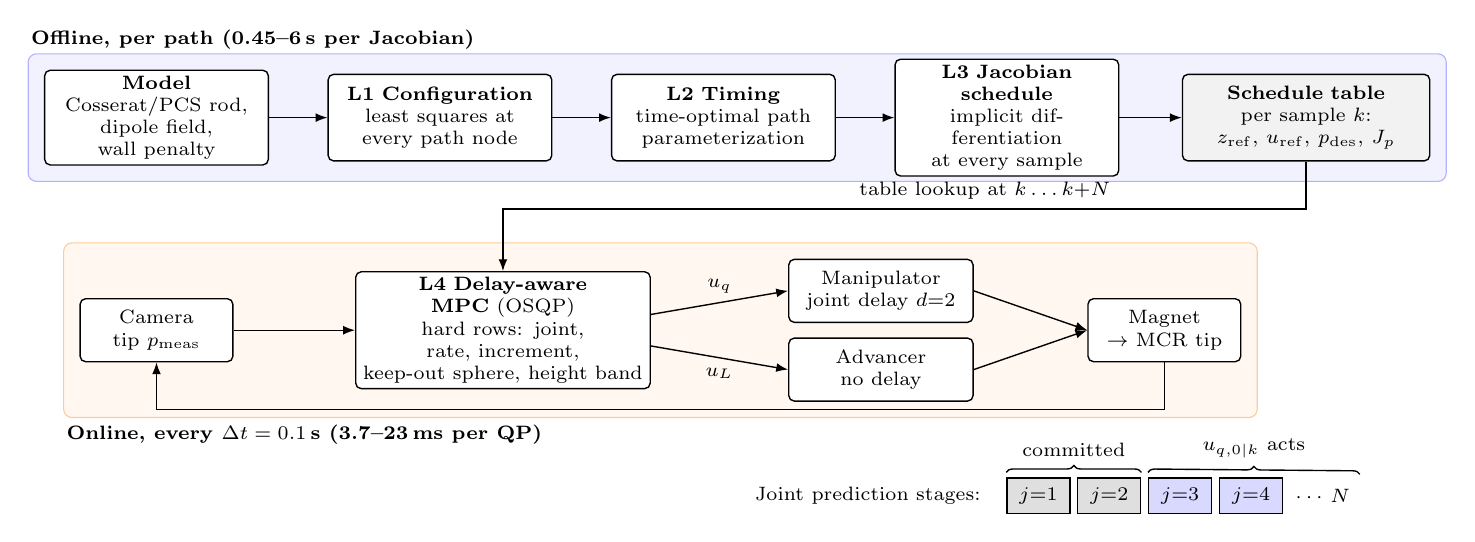
\begin{tikzpicture}[
  font=\scriptsize, >={Latex[length=1.5mm]}, line width=0.5pt,
  lay/.style={draw, rounded corners=2pt, align=center, minimum height=11mm,
              text width=27mm, inner sep=2pt, fill=white},
  on/.style={draw, rounded corners=2pt, align=center, minimum height=8mm,
              inner sep=2pt, fill=white},
  ]
% ---------------- offline lane ----------------
\node[lay] (model) at (0,0) {\textbf{Model}\\Cosserat/PCS rod,\\dipole field, wall penalty};
\node[lay] (l1) at (36mm,0) {\textbf{L1 Configuration}\\least squares at\\every path node};
\node[lay] (l2) at (72mm,0) {\textbf{L2 Timing}\\time-optimal path\\parameterization};
\node[lay] (l3) at (108mm,0) {\textbf{L3 Jacobian schedule}\\implicit differentiation\\at every sample};
\node[lay, text width=30mm, fill=gray!10] (tab) at (146mm,0) {\textbf{Schedule table}\\per sample $k$:\\$z_{\mathrm{ref}},\,u_{\mathrm{ref}},\,p_{\mathrm{des}},\,J_p$};
\draw[->] (model) -- (l1);
\draw[->] (l1) -- (l2);
\draw[->] (l2) -- (l3);
\draw[->] (l3) -- (tab);
\begin{scope}[on background layer]
\node[fill=blue!5, draw=blue!30, rounded corners=3pt, fit=(model)(tab), inner sep=2mm] (offbg) {};
\end{scope}
\node[anchor=south west, font=\scriptsize\bfseries, inner sep=1pt] at (offbg.north west) {Offline, per path (0.45--6\,s per Jacobian)};
% ---------------- online lane ----------------
\node[on, text width=18mm] (cam) at (0,-27mm) {Camera\\tip $p_{\mathrm{meas}}$};
\node[on, text width=36mm] (mpc) at (44mm,-27mm) {\textbf{L4 Delay-aware MPC} (OSQP)\\hard rows: joint, rate, increment,\\keep-out sphere, height band};
\node[on, text width=22mm] (arm) at (92mm,-22mm) {Manipulator\\joint delay $d{=}2$};
\node[on, text width=22mm] (adv) at (92mm,-32mm) {Advancer\\no delay};
\node[on, text width=18mm] (mcr) at (128mm,-27mm) {Magnet\\$\rightarrow$ MCR tip};
\draw[->] (cam) -- (mpc);
\draw[->] ([yshift=2mm]mpc.east) -- node[above]{$u_q$} (arm.west);
\draw[->] ([yshift=-2mm]mpc.east) -- node[below]{$u_L$} (adv.west);
\draw[->] (arm.east) -- (mcr.west);
\draw[->] (adv.east) -- (mcr.west);
\draw[->] (mcr.south) -- ++(0,-6mm) -| (cam.south);
\draw[->] (tab.south) -- ++(0,-6mm) -| node[pos=0.2, above]{table lookup at $k\ldots k{+}N$} (mpc.north);
\begin{scope}[on background layer]
\node[fill=orange!6, draw=orange!40, rounded corners=3pt, fit=(cam)(arm)(adv)(mcr), inner sep=2mm] (onbg) {};
\end{scope}
\node[anchor=north west, font=\scriptsize\bfseries, inner sep=1pt] at ([yshift=-0.5mm]onbg.south west) {Online, every $\Delta t=0.1$\,s (3.7--23\,ms per QP)};
% ---------------- delay inset ----------------
\begin{scope}[shift={(112mm,-48mm)}]
\foreach \j/\c in {1/gray!25,2/gray!25,3/blue!15,4/blue!15} {
  \node[draw, minimum width=8mm, minimum height=4.5mm, fill=\c] (s\j) at ({(\j-1)*9mm},0) {$j{=}\j$};
}
\node[anchor=west] (dots) at ($(s4.east)+(0.3mm,0)$) {$\cdots\,N$};
\draw[decorate,decoration={brace,amplitude=2.5pt}] ([yshift=0.6mm]s1.north west) -- node[above=2pt]{committed} ([yshift=0.6mm]s2.north east);
\draw[decorate,decoration={brace,amplitude=2.5pt}] ([yshift=0.6mm]s3.north west) -- node[above=2pt]{$u_{q,0|k}$ acts} ([yshift=0.6mm]dots.north east);
\node[anchor=east, font=\scriptsize] at ([xshift=-2mm]s1.west) {Joint prediction stages:};
\end{scope}
\end{tikzpicture}
\caption{The framework. Offline layers L1--L3 turn a quasi-static model
into a schedule of reference configurations, rates, tip targets and
Jacobians. Online, L4 reads the tip targets and Jacobians over its horizon
and commands six joints
and insertion under hard constraints; independent monitors (not shown)
re-check the safety bounds from measured joints. Bottom right: because
joint commands act only after $d=2$ ticks, the first predicted stage they
influence is $j=3$.}
\label{fig:framework}
\end{figure*}

\subsection{Platform and Problem Statement}
\label{sec:problem}

A permanently magnetized MCR is advanced through a fixed insertion point
by a linear advancer while a permanent magnet on the end-effector of a
six-axis manipulator shapes it (Fig.~\ref{fig:setup},
Table~\ref{tab:params}). The physical input to the MCR is the magnet pose
and the inserted length, $\theta=[p_a;\phi_a;\ell]\in\mathbb R^7$. Because
the magnet is rigidly mounted, $\theta$ is fixed by the joint angles
$q\in\mathbb R^6$, and the controlled configuration and input are
\begin{equation}
z=[q;\,L]\in\mathbb R^7,\qquad u=\dot z .
\label{eq:config}
\end{equation}
Joint angles are measured; the insertion length $L$ is integrated from the
commanded rate. Given a desired tip path, the problem is to choose $u$ in
real time so that the measured tip follows it, while joints, rates,
accelerations, the magnet's height, and its distance from the insertion
point stay within bounds at every instant. The MCR deforms in a calibrated
plane, and tip position is regulated through a projector
$C\in\mathbb R^{2\times3}$ onto that plane. All quantities are expressed in
the robot-base frame.
% VERIFY: calibration residual of the planner-to-robot transform.

\begin{table}[t]
\centering
\caption{Platform, Model, Controller, and Constraint Parameters}
\label{tab:params}
\footnotesize
\setlength{\tabcolsep}{3.5pt}
\begin{tabular}{@{}ll@{}}
\toprule
\multicolumn{2}{@{}l}{\emph{Platform}} \\
Manipulator & UR10e, External Control URCap \\
Control computer & i7-11700K, 31\,GB RAM \\
Operating system & Ubuntu 22.04, PREEMPT\_RT kernel \\
Command stream / control period & 125\,Hz / $\Delta t=0.1$\,s \\ % VERIFY 125 Hz
Joint / insertion delay $d$ & 2 / 0 ticks \\
Advancer resolution & 0.166\,mm/step \\
\midrule
\multicolumn{2}{@{}l}{\emph{MCR and magnet model}} \\
MCR diameter / PCS nodes $n_s$ & 2.0\,mm / 10 \\
Effective modulus $E$ / Poisson $\nu$ & $\approx$2.5\,MPa / 0.49 \\ % VERIFY core wire, fit residual
Magnet & N52 NdFeB cylinder, $100\times100$\,mm \\ % VERIFY dipole moment
Wall $k_c$ / $\varepsilon_c$ & $10^{8}$\,N\,m$^{-2}$ / $10^{-5}$\,m \\ % AUTHOR CHECK units against the code's definition of W_c
\midrule
\multicolumn{2}{@{}l}{\emph{MPC and baseline}} \\
Horizon $N$ & 15 (ablated: 3, 1) \\
$Q_p$ / $R$ / $R_d$ (normalized) & 1.0 at 0.5\,mm / 7.0 / $10^{-3}$ \\ % config input_tracking_weight = 7.0; variant name "R700" = 700 R_0 if R_0 = 0.01: confirm R_0 and drop the R700 label
Null-space posture weight $\gamma$ & 0 (all experiments) \\
$S_u$ (joint / insertion) & 0.05\,rad/s / 5\,mm/s \\
$S_{\Delta u}$ (joint / insertion) & 0.04\,rad/s / 2\,mm/s \\
INV-7 $k_p$ / $k_n$ / $\lambda_u$ & 1.0 (and 0.6) / 0 / $2.5\times10^{-3}$ \\
\midrule
\multicolumn{2}{@{}l}{\emph{Hard constraints in the QP}} \\
Joint / insertion velocity & 0.10\,rad/s / 2\,mm/s \\
Joint / insertion acceleration & 0.40\,rad/s$^2$ / 20\,mm/s$^2$ \\
Joint / insertion position & \TBD{joint box} / \TBD{insertion range} \\
Magnet keep-out sphere (vessel) & 235\,mm about insertion point \\ % AUTHOR CHECK: centre = insertion point
Magnet height from start (vessel) & $-28.1$ to $16.9$\,mm \\
TCP box $x$; $y$; $z$ (m) & $0.27$--$0.66$; $-0.75$--$-0.53$; $0.17$--$0.50$ \\
Tracking-error abort (MPC / INV-7) & 7.0 / 15\,mm \\
\bottomrule
\end{tabular}
\end{table}

% =============================================================
\section{Offline Layers: Model, Configuration, Timing, and Jacobians}
\label{sec:offline}
% =============================================================

\subsection{Quasi-Static Magnetic Rod Model}
\label{sec:model}

The MCR is a Cosserat rod of inserted length $\ell$ under a
piecewise-constant-strain (PCS) discretization~\cite{renda2018discrete},
with strain $u(s)$ constant on each of $n_s$ segments and stiffness
$K=\operatorname{diag}(GI_p,EI,EI)$. The magnet, of moment $m_a$, is
modeled as a point dipole. With $\Delta=x-p_a$, $r=\lVert\Delta\rVert$,
$\hat\Delta=\Delta/r$, and $m(s)$ the MCR's body-frame magnetization per
unit length,
\begin{align}
B(x;\theta)&=\frac{\mu_0}{4\pi r^3}\big[3(\hat\Delta^\top m_a)\hat\Delta-m_a\big],
\label{eq:dipole}\\
W_m&=-\int_0^\ell\big(R(s)m(s)\big)^{\!\top}B\big(p(s);\theta\big)\,ds,
\label{eq:wm}
\end{align}
where $(p(s),R(s))$ follows from $p'=Re_3$, $R'=R\hat u$. The field, and
therefore the magnetic load, changes in magnitude and direction along the
MCR and with every joint motion; it is never uniform over the workspace.
In the vessel, the lumen wall enters as a smooth penalty
$W_c=\int_0^\ell\frac12k_c\varphi_+^2\,ds$ on the smoothed penetration
$\varphi_+$ of the rod into the wall. How the wall changes the Jacobian is
analysed in a companion study; here it is one module of the model. With
elastic energy $W_{el}$ about the rest strain and gravitational energy
$W_g$, the equilibrium is
\begin{equation}
u^*(\theta)=\arg\min_u\ \Pi(u;\theta),\qquad
\Pi=W_{el}+W_m+W_g+W_c,
\label{eq:equilibrium}
\end{equation}
solved by L-BFGS-B~\cite{byrd1995lbfgsb} on analytic gradients,
warm-started along $\ell$ so that the solution follows the branch reached by
incremental insertion. $W_g$ and $W_c$ vanish on the horizontally
supported free-space paths.

\subsection{L1: Configuration at Every Path Node}
\label{sec:l1}

The first layer converts a desired tip path into a feasible configuration
at each node. Configurations $\chi_j=[q;\ell]_j$ are found sequentially by
nonlinear least squares on
\begin{equation}
\begin{aligned}
r(\chi_j)=\Big[&\tfrac{p_{\mathrm{tip}}(\chi_j)-p_{\mathrm{des},j}}{\tau_p};\,
\tfrac{t_{\mathrm{tip}}(\chi_j)-t_{\mathrm{des},j}}{\tau_t};\\
&\sqrt{w_c}\,\tfrac{\chi_j-\chi_{j-1}}{d_c};\,
\sqrt{w_0}\,\tfrac{\chi_j-\chi_0}{d_0}\Big],
\end{aligned}
\label{eq:planner}
\end{equation}
whose blocks penalize tip position and tangent error, discontinuity with
the previous node, and departure from a nominal posture $\chi_0$ that
resolves the arm's redundancy. Each node is warm-started from its
predecessor, restarted when the solve fails, and accepted only after
verification against the full model~\eqref{eq:equilibrium}.
% AUTHOR CHECK: report tau_p, tau_t, w_c, d_c, w_0, d_0 and the accepted
% residual; without code release these are needed for reproducibility.

\subsection{L2: Time Parameterization}
\label{sec:l2}

The second layer assigns timing. The node sequence is parameterized by
reachability-based time-optimal path
parameterization~\cite{bobrow1985timeoptimal,shinmckay1985minimumtime,
phampham2018reachability}: a backward pass computes the controllable set
and a forward pass the fastest feasible speed profile under the joint and
insertion velocity and acceleration limits of Table~\ref{tab:params}. The
profile is smoothed by a $C^2$ spline and dilated to a whole number of
control periods, so that reference sample $k$ coincides with control tick
$k$. The output is $z_{\mathrm{ref},k}$, the feedforward rate
$u_{\mathrm{ref},k}$, and the tip target $p_{\mathrm{des},k}$.

\subsection{L3: Jacobian Schedule by Implicit Differentiation}
\label{sec:l3}

The third layer computes, at every reference sample, how each joint and the
insertion move the tip. Differentiating the equilibrium condition
$\nabla_u\Pi(u^*;\theta)=0$ gives
\begin{equation}
\frac{\partial u^*}{\partial\theta}=-\Pi_{uu}^{-1}\Pi_{u\theta},\qquad
J_b=\frac{\partial y}{\partial u}\frac{\partial u^*}{\partial\theta}
+\frac{\partial y}{\partial\theta}\Big|_{u^*},
\label{eq:ift}
\end{equation}
with $y$ the tip pose and the Hessian blocks finite-differenced from the
analytic gradient, so no equilibrium is re-solved under perturbation.
Composing with the manipulator Jacobian $J_r(q)$~\cite{lynchpark2017modern}
gives the joint-space Jacobian $J(z)=J_b\operatorname{blkdiag}(J_r,1)$ and its
position block $J_p\in\mathbb R^{3\times7}$. The schedule is
\begin{equation}
J_{p,k}=J_p(z_{\mathrm{ref},k}),\qquad k=0,\dots,K,
\label{eq:schedule}
\end{equation}
stored with the reference. Each $J_{p,k}$ costs 0.45--0.48\,s on the
free-space paths and 0.89--6.0\,s on the vessel, rising as the rod
approaches the wall (Table~\ref{tab:compute}), which is 5--60 times the
control period. On the vessel, the stored schedule combines the
wall-aware model's joint columns with the free-lumen insertion column.
The free-space schedules were computed in a faster solver setting; at
spot-checked samples they agreed with the accurate setting within 1\%,
with one sample at 7\%, and showed no spurious singular-value spikes.
Against finite differences of the same model in joint space, the
schedule agrees within 2.2\% on average (5.9\% at most) on the triangle
and 4.1\% (15.6\%) on the rectangle, and within 9.3\% at all 20 checked
states along the vessel path. Near the wall the finite-difference step must
be at least $10^{-3}$\,rad; smaller steps fall below the equilibrium
solver's tolerance and give spurious errors.
% AUTHOR CHECK: re-run the free-space comparison with the same step rule;
% the 15.6% rectangle maximum may be the same artifact.
% AUTHOR CHECK: state what the fast setting changes (tolerances? FD step?)
% and how many samples were spot-checked. The hybrid vessel schedule is
% analysed in the companion paper; give one sentence of rationale here.
The single-magnet system offers few independent steering directions, so
$J_p$ is poorly conditioned over much of each path: its condition number
ranges from 4.7 to 208 across paths, with medians of 11.5--23.0.

\begin{algorithm}[t]
\caption{Offline--online framework}
\label{alg:framework}
\footnotesize
\begin{algorithmic}[1]
\Statex \textbf{Offline} (per path)
\For{each path node $j$}
  \State $\chi_j\gets\arg\min\lVert r(\chi_j)\rVert^2$ from $\chi_{j-1}$ \Comment{L1, \eqref{eq:planner}}
  \State verify $\chi_j$ with the full model \eqref{eq:equilibrium}
\EndFor
\State $\{z_{\mathrm{ref},k},u_{\mathrm{ref},k},p_{\mathrm{des},k}\}\gets$ TOPP-RA$(\chi)$ \Comment{L2}
\For{each sample $k$}
  \State $J_{p,k}\gets$ implicit derivative at $z_{\mathrm{ref},k}$ \Comment{L3, \eqref{eq:ift}}
\EndFor
\Statex \textbf{Online} (every $\Delta t$)
\State read $p_{\mathrm{meas},k}$, $q_k$; integrate $L_k$; form $d_k$ \Comment{\eqref{eq:residual}}
\State build prediction \eqref{eq:delay}--\eqref{eq:pred} from $J_{p,k\ldots k+N}$
\State linearize keep-out and height constraints at each stage
\State solve QP \eqref{eq:mpc}; on deadline miss hold $c_k$ \Comment{L4}
\State $c_{k+1}\gets c_k+\Delta t\,u_{0|k}$; stream to arm and advancer
\State re-check bounds from measured joints; stop on violation
\end{algorithmic}
\end{algorithm}

% =============================================================
\section{Online Layer: Delay-Aware Constrained MPC}
\label{sec:online}
% =============================================================

\subsection{Delay-Aware Prediction}
\label{sec:pred}

The online layer predicts the tip from the schedule rather than the model.
With $J_{\mathrm{task},k}=CJ_{p,k}$, a new joint command first affects the
commanded joint position $d=2$ ticks later, while insertion responds at
once. With $c_k$ the committed joint command and $u_{q,r|k}$ the joint rate
chosen for stage $r$,
\begin{equation}
q_{j|k}=
\begin{cases}
c_{k-1}, & j=1,\\
c_{k}, & j=2,\\
c_k+\Delta t\sum_{r=0}^{j-3}u_{q,r|k}, & j\ge3,
\end{cases}
\label{eq:delay}
\end{equation}
and $L_{j|k}=L_k+\Delta t\sum_{r=0}^{j-1}u_{L,r|k}$. Stage $j=d+1=3$ is the
first that a new joint command can influence (Fig.~\ref{fig:framework},
inset); a horizon $N\le d$ contains none. The per-tick residual
\begin{equation}
d_k=Cp_{\mathrm{meas},k}-\big[Cp_{\mathrm{des},k}
+J_{\mathrm{task},k}(z_{\mathrm{meas},k}-z_{\mathrm{ref},k})\big]
\label{eq:residual}
\end{equation}
is held constant over the horizon~\cite{maeder2009linear}, giving, with $\delta z_{j|k}=z_{j|k}-z_{\mathrm{ref},k+j}$,
\begin{equation}
\hat p_{j|k}=Cp_{\mathrm{des},k+j}+J_{\mathrm{task},k+j}\,
\delta z_{j|k}+d_k,
\label{eq:pred}
\end{equation}
Each stage uses its own scheduled Jacobian, so the prediction follows the
change of the control map along the path. As a model-staleness control,
the frozen-Jacobian (FJ) condition replaces every $J_{p,k}$ by the
Jacobian at the start of the trial: at the plan's first sample on the
free-space paths, and at the measured start configuration on the vessel,
which differ by about $10^{-4}$ in relative terms.

\subsection{Constrained Quadratic Program}
\label{sec:mpc}

The MPC chooses $U=[u_{0|k};\dots;u_{N-1|k}]$, with
$\Delta u_{j|k}=u_{j|k}-u_{j-1|k}$ and $u_{-1|k}=u_{k-1}$, by solving
\begin{equation}
\begin{aligned}
\min_U\ &\sum_{j=1}^{N}\lVert\hat p_{j|k}-Cp_{\mathrm{des},k+j}\rVert_{Q_p}^2\\
&+\sum_{j=0}^{N-1}\Big(\lVert u_{j|k}-u_{\mathrm{ref},k+j}\rVert_R^2
+\lVert\Delta u_{j|k}\rVert_{R_d}^2\Big)\\
\text{s.t.}\ & u_{\min}\le u_{j|k}\le u_{\max},\quad
\Delta u_{\min}\le\Delta u_{j|k}\le\Delta u_{\max},\\
& z_{\min}\le z_{j|k}\le z_{\max},\quad
g(z_{j|k})\le0,\qquad \text{all stages}.
\end{aligned}
\label{eq:mpc}
\end{equation}
The input penalty pulls each commanded rate toward the planned rate, so
the plan acts as a feedforward inside the QP, where the constraints apply
to the total command; the controller departs from the planned rates only
where tracking requires it. The command streamed to the arm is a position
accumulator seeded at the measured start configuration,
$c_{k+1}=c_k+\Delta t_k\,u_{0|k}$, where $\Delta t_k$ is the measured tick
period; the arm realizes 96--99\% of each commanded step.
% Confirmed for the vessel and the free-space controller classes: the
% zero-reference diagnostic flag is read by neither, so every hardware run
% used this form.
The box rows encode the manipulator's and advancer's physical limits. The
safety rows $g$ keep the magnet outside a 235\,mm sphere centred on the
insertion point, which protects the patient's access site, and inside a
height band; an optional box bounds the tool center point. Because the
magnet position is a nonlinear function of $q$, each safety row is a
first-order expansion of the magnet's forward kinematics, so the program
remains a QP. The safety rows act on the commanded joint positions
$c_{k+j}$, which the arm reaches $d$ ticks later, so a feasible plan keeps
the physical trajectory inside the same bounds. The TCP box is part of
the QP by default.
% AUTHOR CHECK: (1) state the linearization point (reference, previous
% solution, or measured state). (2) The TCP-in-QP flag was not logged for
% the frozen-Jacobian vessel runs; log argv in all new runs. (3) OSQP
% "solved inaccurate" and accepted time-limited solves are treated as
% success: report their counts.
A null-space posture term can be added to \eqref{eq:mpc}; it was disabled
in every experiment reported here. The QP is solved by OSQP~\cite{osqp2020}
in a pre-warmed, process-isolated worker with a 70\,ms deadline; on a miss
the previous position is held rather than a stale solution applied. Only
$u_{0|k}$ is applied and integrated into a persistent position command
$c_{k+1}=c_k+\Delta t\,u_{0|k}$ streamed to the arm. Independently of the
QP, the magnet's distance and height are recomputed every tick from the
measured joints, the tool center point is monitored in a second frame, and
an insertion-offset monitor (5\,mm) runs; any violation stops the trial.
No stability guarantee is claimed for the nonlinear plant.

\subsection{Baseline: Matched-Authority Inverse-Jacobian Control}
\label{sec:inv7}

To isolate the contribution of in-QP constraints, the baseline INV-7
uses the same model, schedule, delay compensation and actuator limits.
 It targets the first causally affected
reference sample $\kappa_k=r_k+1+d$ and applies one damped least-squares
step~\cite{nakamura1986inverse,wampler1986manipulator,chiaverini1994review},
\begin{equation}
\delta z_k=S_uJ_u^\top\big(J_uJ_u^\top+\lambda_u^2I\big)^{-1}k_p\,e_{\kappa},
\qquad J_u=J_{\mathrm{task},\kappa}S_u,
\label{eq:inv7}
\end{equation}
where $e_\kappa$ is the error predicted at $\kappa_k$ through
\eqref{eq:pred}. Rate and acceleration limits are applied by clipping the
resulting command. The safety bounds are not part of the correction:
before a command is sent, the bounds are checked, and a command that would
break one is blocked, so the magnet holds its position for that tick. The
gain $k_p=1.0$ was chosen to place INV-7 in the same rate-limit saturation
regime as the MPC, not at its most accurate setting: on a predecessor
controller, $k_p=0.6$ gave lower error without saturation, whereas
$k_p=1.0$ saturated on 20.5\% of ticks. Because the comparison concerns
constraint handling rather than tuning, INV-7 is run at this setting
throughout. % AUTHOR CHECK: confirm the blocking rule (zeroed command =
% hold) and the bounds it checks.
% AUTHOR CHECK: lambda_u = 2.5e-3 vs the inherited damping 5e-2 (= sqrt of
% 2.5e-3); make the equation and the table use the same symbol.

% =============================================================
\section{Experimental Design}
\label{sec:experiments}
% =============================================================

\subsection{Questions and Predictions}
\label{sec:questions}

The evaluation tests one claim per layer. Each experiment varies a single
factor, and its prediction was written down before the trials were run.
\begin{itemize}
\item[Q1] \emph{Is a Jacobian schedule needed?} One Jacobian should fail
where the control map changes along the path. Prediction: the error of
the frozen-Jacobian controller relative to the scheduled one grows with
the Jacobian variation of the path, and is decisive on the vessel.
\item[Q2] \emph{Must constraints sit inside the optimizer?} A controller
that checks bounds only after computing its command issues commands that
must be blocked. Prediction: on paths that run close to a bound, INV-7 is
repeatedly frozen and fails, while the MPC tracks along the bound.
\item[Q3] \emph{What does a long horizon buy?} A horizon shorter than the
delay cannot steer the joints at all. Beyond that, the expected benefit
is not finer accuracy but anticipation: a minimal horizon commits the
magnet toward a bound it sees too late to avoid under the rate and
acceleration limits. Prediction: on paths that approach a bound at speed
and then turn, MPC at $N=3$ becomes infeasible or is stopped, while
$N=15$ completes.
\end{itemize}

\subsection{Tasks and Conditions}
\label{sec:tasks}

\emph{Vessel.} The vessel task follows the digitized centerline of a
\TBD{material, fabrication, planar or 3-D} phantom (lumen radius
\TBD{range}) on plan B, which includes a dipole-alignment term in L1; plan
B$'$ omits that term. % AUTHOR CHECK: define the dipole-alignment term.
Segment C ($55\le s\le65$\,mm) is the highest-curvature part of the path.
The plan keeps the magnet within a few millimetres of its height band:
the minimum clearance of the reference is \TBD{3.4}\,mm, and \TBD{42.7}\% of its
samples lie within 5\,mm. It therefore tests Q1--Q3 under realistic
constraints.

\emph{Free-space paths for Q1.} A $15\times10$\,mm rectangle and an
isosceles triangle at three base widths, 25\,mm and \NEWRUN{$W_2$,
$W_3$}\,mm. The widths were chosen offline, before any trial, so that the
late-path Jacobian variation $V_k$ increases with width
(Section~\ref{sec:metrics}).

\emph{Trap paths for Q3.} Free-space paths on which the planned magnet
trajectory approaches the height band or keep-out sphere and must then
turn away. Two parameters set how hard the task is: the reference speed,
as a fraction $\alpha\in\{\NEWRUN{0.6, 0.8, 1.0}\}$ of the time-optimal
profile from L2, and the planned clearance to the bound,
$\delta\in\{\NEWRUN{10, 5, 2}\}$\,mm. The full grid was first simulated
with a perturbed plant; \NEWRUN{three} points were then run on hardware: one
where both horizons were predicted to succeed, one where only $N=15$
was, and one where both were predicted to fail.

\emph{Silicone model.} A silicone model of \NEWRUN{vessel segment and
source, e.g., a segmented internal carotid--middle cerebral artery} is
the final demonstration; it was not used in any tuning.

\emph{Conditions.} Table~\ref{tab:conditions} lists the trials. MPC at
$N=d+1=3$ plays a specific role: its joint commands affect exactly one
predicted stage, so it is the constrained counterpart of INV-7 and differs
from $N=15$ only in lookahead. MPC at $N=1$ contains no stage the joints
can reach and is reported as an ablation of joint feedback. Trials of
different conditions were \NEWRUN{interleaved in randomized order} within
each session, and the vessel $N=15$ condition was repeated in the same
session as $N=3$ so that both run at the same realized period.
% AUTHOR CHECK: existing rectangle runs were blocked by condition; report
% a drift check for them.

\begin{table}[t]
\centering
\caption{Conditions and Trials per Task}
\label{tab:conditions}
\footnotesize
\setlength{\tabcolsep}{2.5pt}
\begin{tabular}{@{}lcccc@{}}
\toprule
Condition & Rect. & Triangle (3 widths) & Trap & Vessel B \\
\midrule
Feedforward only & 10 & 10, ---, --- & --- & --- \\
INV-7, SJ        & 10 & 10, ---, --- & \NEWRUN{3$\times$5} & 16 + 11 \\
MPC, FJ, $N=15$  & 10 & 10, \NEWRUN{10, 10} & --- & 16 \\
MPC, SJ, $N=15$  & 10 & 10, \NEWRUN{10, 10} & \NEWRUN{3$\times$10} & 10 + \NEWRUN{10} \\
MPC, SJ, $N=3$   & \NEWRUN{10} & --- & \NEWRUN{3$\times$10} & \NEWRUN{10} \\
MPC, SJ, $N=1$   & 10 & 10 & --- & 10 \\
MPC, FJ, $N=1$   & 10 & 10 & --- & --- \\
\bottomrule
\end{tabular}

\vspace{2pt}
\parbox{\columnwidth}{\footnotesize Vessel entries for INV-7 and MPC-FJ
are attempted trials; INV-7 ran with the MPC's schedule (16) and with a
fully wall-aware schedule (11). Plan B$'$ repeats MPC-SJ at $N=15$ and
$N=1$ ($2\times10$) and INV-7 (16). The silicone model is run with MPC-SJ
at $N=15$ only (\NEWRUN{$n$} trials). INV-7 with a frozen Jacobian on the
free-space paths is reported in the supplementary material.}
\end{table}

\subsection{Metrics and Statistics}
\label{sec:metrics}

Tracking error at tick $k$ is $e_k=C(p_{\mathrm{meas},k}-p_{\mathrm{des},r_k})$
with the logged reference index $r_k$; accuracy is the trial-level
$E_{\mathrm{RMS}}=(\frac1T\sum_k\lVert e_k\rVert^2)^{1/2}$, split into lag
and cross-track components where stated. Completion is reported alongside
accuracy, and a trial stopped by a safety monitor or error limit counts as
a failure with its cause. A trial is \emph{trapped} if its QP is
infeasible, or its command is held, for at least \NEWRUN{5} consecutive
ticks. For INV-7 we count \emph{frozen} ticks, at which its command was
blocked because it would have broken a bound. The trial is the
experimental unit; tables give the trial-level mean $\pm$ 95\% CI or
median and range. Groups are compared by the two-sided Mann--Whitney $U$
test~\cite{mann1947test} (with $n=10$, the asymptotic $p$ cannot fall
below $1.8\times10^{-4}$, the value reported for complete separation), by
Fisher's exact test for completion counts, and by exact permutation tests
where stated, with Holm correction~\cite{holm1979simple}.

\emph{Sensing.} An overhead camera tracks colored markers on the MCR,
segmented by HSV thresholding; three proximal markers define the
deformation plane by principal component analysis, and a marker pair of
known 38\,mm separation sets metric scale~\cite{shi2017shape}. The tip
estimate is not filtered and reaches the controller with a mean age of
30.5\,ms. Because the MCR moves slowly relative to the 0.1\,s tick,
random measurement noise is bounded from above by the tick-to-tick second
difference of the measured tip, $\sigma\le\mathrm{std}(\Delta^2p)/\sqrt6$,
which gives 0.135\,mm for the in-plane position (0.125 and 0.178\,mm
along the two axes) over 20 open-loop free-space trials. This bounds
frame-to-frame jitter only, not systematic calibration error.

\emph{Jacobian variation.} Along each reference we measure the relative
change $V_k=\lVert J_{p,k}-J_{p,0}\rVert_F/\lVert J_{p,0}\rVert_F$ and the
condition number of $J_{p,k}$.

\emph{Constraint activity.} From the live logs of each trial we report
the fraction of ticks at which the magnet sits on a safety bound, the
solver status, and the minimum clearance to the keep-out sphere and
height band.

\emph{Offline replay.} Same-state replay re-solves the controller offline
at logged states. It reproduces the live command closely but not
exactly: the cosine between replayed and live commands has a median of
0.988 (10th percentile 0.893) and exceeds 0.999 on 35\% of ticks, so
replay results are used only as supporting evidence and none of the main
results depends on them.

% =============================================================
\section{Results}
\label{sec:results}
% =============================================================

\subsection{Real-Time Performance}
\label{sec:res-time}

The offline--online split is what makes the model usable in the loop
(Table~\ref{tab:compute}). A single scheduled Jacobian takes 0.45\,s on a
free-space path and up to 6\,s near the vessel wall; the full schedule for
a vessel plan takes 336--3217\,s. Online, the QP solves in 3.7\,ms on
average on the rectangle (7.4\,ms maximum) and 20--23\,ms on the vessel at
$N=15$, so every solve fits the 100\,ms control period with margin; 2.7\%
of vessel solves reached the solver's time limit. State estimates are
30.5\,ms old on average (70.6\,ms maximum). The realized period on the
vessel was 105.6\,ms at $N=1$ and 125.3\,ms at $N=15$
\TBD{cause of the overrun}. The reference advances one sample per tick,
so a longer period slows execution; but the command accumulator integrates
over the measured period while the prediction assumes 0.1\,s, so each
command also moves the arm 6\% (at $N=1$) to 25\% (at $N=15$) further
than predicted, an error the feedback must absorb. In the new trials the
realized period was \NEWRUN{100\,ms} at $N=15$.
% AUTHOR CHECK: the scheduler is reported as drift-free (next_tick += dt),
% which should NOT add the solve time to the period. Recompute the period
% from logged tick timestamps and find what produces the 25 ms overrun
% before stating a cause. Reconcile 2.7% "time-limit hits" with the 0.16%
% of ticks at the ~70 ms deadline; state whether d = 2 was identified at
% the 100 ms or the realized period.

\begin{table}[t]
\centering
\caption{Computation of Each Layer}
\label{tab:compute}
\footnotesize
\setlength{\tabcolsep}{3pt}
\begin{tabular}{@{}lll@{}}
\toprule
Layer & Task & Time \\
\midrule
L1 configuration & rectangle / triangle & 997 / 1666\,s \\
                 & vessel & 9983\,s \\
L2 timing & rectangle / triangle / vessel & 79 / 112 / 335\,s \\
L3 Jacobian & rectangle (209 samples) & 0.45\,s/sample; 95\,s \\
            & triangle (288 samples)  & 0.48\,s/sample; 138\,s \\
            & vessel, free-lumen (378) & 0.89\,s/sample; 336\,s \\
            & vessel, wall-aware (534--578) & 3.0--6.0\,s/sample; \\
            &                              & 1747--3217\,s \\
\midrule
L4 QP solve & rectangle, $N=15$ & 3.7\,ms mean, 7.4\,ms max \\
            & vessel, $N=15$ / $N=1$ & 20--23\,ms / 4.5\,ms mean \\
            & vessel deadline hits & 150/5513 (2.7\%) / 0/6367 \\
State age & all trials & 30.5\,ms mean, 70.6\,ms max \\
Realized period & vessel, $N=1$ / $N=15$ & 105.6 / 125.3\,ms \\
                & new trials, $N=15$ & \NEWRUN{100\,ms} \\
\bottomrule
\end{tabular}
\end{table}

\subsection{Tracking With the Full Framework}
\label{sec:res-track}

The full framework tracked both free-space paths to sub-millimetre
accuracy and completed every vessel trial (Tables~\ref{tab:shape}
and~\ref{tab:vessel}). The offline layers alone, applied as feedforward,
left 1.81\,mm of error on the rectangle and 1.54\,mm on the triangle;
closing the loop with the MPC reduced it to 0.46 and 0.80\,mm.
On the vessel, MPC with the scheduled Jacobian
completed 10 of 10 trials at a median error of 0.708\,mm (range
0.626--0.786), and reproduced this on plan B$'$ (median 0.66--0.68\,mm).

\begin{table}[t]
\centering
\caption{Free-Space Tracking: Trials Completed of 10, and $E_{\mathrm{RMS}}$
in mm (Mean $\pm$ 95\% CI over Completed Trials)}
\label{tab:shape}
\footnotesize
\setlength{\tabcolsep}{2.5pt}
\begin{tabular}{@{}lcccc@{}}
\toprule
 & \multicolumn{2}{c}{Rectangle} & \multicolumn{2}{c}{Triangle (25\,mm)} \\
Condition & Done & $E_{\mathrm{RMS}}$ & Done & $E_{\mathrm{RMS}}$ \\
\midrule
Feedforward only   & 10 & $1.811\pm0.197$ & 10 & $1.536\pm0.098$ \\
INV-7, SJ          & 10 & $0.600\pm0.030$ & 10 & $0.876\pm0.094$ \\
INV-7, FJ          & 10 & $1.183\pm0.325$ & 10 & $0.910\pm0.032$ \\
MPC, FJ, $N=15$    & 3$^\ast$ & $0.963\pm0.008$ & 10 & $0.627\pm0.018$ \\
MPC, SJ, $N=15$    & 9$^\ddagger$ & $0.457\pm0.032$ & 10 & $0.801\pm0.052$ \\
MPC, SJ, $N=3$     & \NEWRUN{} & \NEWRUN{} & --- & --- \\
MPC, SJ, $N=1$     & 10 & $1.798\pm0.166$ & 10 & $1.073\pm0.042$ \\
MPC, FJ, $N=1$     & 10 & $1.877\pm0.146$ & 10 & $1.263\pm0.047$ \\
\bottomrule
\end{tabular}

\vspace{2pt}
\parbox{\columnwidth}{\scriptsize Trials are the first valid attempt of
each of 10 repetitions. An attempt stopped by the insertion-offset
monitor, which was not part of the protocol, was treated as interrupted
and repeated; this replaced 4 rectangle FJ and 6 triangle SJ attempts
(supplementary material). No completed trial in any condition reached the
monitor's 5\,mm threshold. $^\ast$The other 7 stopped at the TCP box.
$^\ddagger$1 stopped at the TCP box.}
% Rule as applied: the attempt replacing an interrupted one is the trial,
% whatever its outcome (rectangle FJ rep 4: interrupted, then TCP box).
% AUTHOR CHECK: confirm 0.963 +/- 0.008 (n=3) is over the three trials of
% the current trial set (reps 5-7 repeats), with a t-based CI (t=4.30).
\end{table}

\begin{table}[t]
\centering
\caption{Vessel Navigation, Plan B: $E_{\mathrm{RMS}}$ in mm}
\label{tab:vessel}
\scriptsize
\setlength{\tabcolsep}{2pt}
\begin{tabular}{@{}lccccc@{}}
\toprule
Condition & Done & Median & Range & Lag / cross & Clearance \\
\midrule
MPC, SJ, $N=15$ & 10/10 & 0.708 & 0.626--0.786 & 0.508 / 0.436 & \NEWRUN{} \\
MPC, SJ, $N=1$  & \TBD{0/14}$^{\S}$ & 2.207 & 2.035--2.483 & 1.111 / 1.911 & \NEWRUN{} \\
MPC, FJ, $N=15$ & 0/16$^{\ast}$ & --- & --- & --- & --- \\
INV-7, SJ & 0/14$^{\dagger}$ & --- & --- & --- & --- \\
\midrule
\multicolumn{6}{@{}l}{\emph{New session, interleaved}} \\
MPC, SJ, $N=15$ & \NEWRUN{} & \NEWRUN{} & \NEWRUN{} & \NEWRUN{} & \NEWRUN{} \\
MPC, SJ, $N=3$  & \NEWRUN{} & \NEWRUN{} & \NEWRUN{} & \NEWRUN{} & \NEWRUN{} \\
\bottomrule
\end{tabular}

\vspace{2pt}
\parbox{\columnwidth}{\scriptsize Lag and cross-track are median RMS
components; clearance is the minimum distance to the keep-out sphere over
all trials of a condition. Counts are attempts, including attempts
repeated after an abort, over 10 repetitions per condition. Stops:
$^\ast$10 tracking error, 3 keep-out, 3 TCP box; $^\dagger$10 tracking
error, 4 height band (upper bound), excluding one attempt run at a 7\,mm
abort limit and one software crash; $^\S$all 14 reached the final
reference sample and were then stopped by the 7\,mm error limit
\TBD{completion rule}. Diagnostic INV-7 runs with a fully wall-aware
schedule are in the supplementary material.
INV-7 aborted at 15\,mm tracking error (one trial at 7\,mm), the MPC at
7\,mm.}
\end{table}

\begin{figure*}[t]
\centering
\figph{\textwidth}{4.4cm}{Measured tip paths over the reference: (a)
rectangle, (b) triangle at the three widths, one median trial each for
MPC-FJ and MPC-SJ at $N=15$ (plus feedforward and INV-7-SJ on the
rectangle and 25\,mm triangle), corners enlarged;
(c) vessel, MPC-SJ at $N=15$ with segment C marked and the point where
each INV-7 and MPC-FJ trial stopped.}
\caption{Tip paths on the free-space and vessel tasks.}
\label{fig:paths}
\end{figure*}

\subsection{Q1: The Jacobian Schedule}
\label{sec:res-jac}

One Jacobian could not carry the vessel task: with the Jacobian frozen at
the start, the MPC completed none of its 10 trials (none of 16 valid
attempts), against 10 of 10 with the schedule
(Table~\ref{tab:vessel}; Fisher $p=1.1\times10^{-5}$). Simulation shows why:
with the vessel model as both plant and predictor, the frozen Jacobian
accumulates 4.9 times more prediction error than the schedule by stage
$j=15$ (0.397 vs.\ 0.082\,mm, Fig.~\ref{fig:prediction}), and in a paired
closed-loop Monte Carlo over initial-state perturbations, scheduling
reduced tracking error by 4.31\,mm (95\% CI 4.15--4.47) in 10 of 10
seeds.
% AUTHOR CHECK: justify the sigma = 2 deg joint perturbation.
These are not solver failures. Live, the frozen-Jacobian QP returned a
normal solution on a median 97.5\% of ticks per attempt (range
95.1--99.3\%); its commands were feasible but computed from a stale map.
Late in the path the frozen Jacobian understates the effect of the three
dominant joints on the tip by a factor of 13--17, while its insertion
column stays close to the schedule's. To the frozen controller, joint
motion therefore looks expensive for little benefit, and it
under-corrects: it commanded less joint motion per millimetre of error
than the scheduled controller (median 0.023, range 0.015--0.072,
against 0.031, range 0.028--0.033\,rad\,s$^{-1}$\,mm$^{-1}$ on the three
dominant joints), its commands rarely reversed (5.5\% of late-path ticks,
range 0--16.2\%, against 23.9\%, range 20.5--26.9\%), and the error grew
smoothly until the 7\,mm limit stopped \TBD{$m$} of the 10 trials.
% Offline re-solves of the FJ runs disagree with the live status after the
% first ~15% of each trial (warm-start drift); do not use offline-replay
% infeasibility or binding fractions for FJ anywhere.

\begin{figure}[t]
\centering
\includegraphics[width=\columnwidth]{figures/fig_prediction_horizon.pdf}
\caption{Simulated tip prediction error along the horizon on the vessel
path with the initial (frozen) and scheduled Jacobians, averaged over 11
starting ticks.}
\label{fig:prediction}
\end{figure}

On the free-space paths the frozen Jacobian's error depended on how far
the map moved from where it was frozen. On the rectangle the MPC
completed 9 of 10 trials with the schedule and 3 of 10 with the frozen
Jacobian, whose other seven stopped at the TCP box; every frozen trial broke
down late in the path, with a last-third error of 3.9\,mm before its stop,
where $V_k$ has grown from 0.06 to 0.63. In completed trials the two
controllers were indistinguishable over the first two thirds of the path
(median 0.41 against 0.38\,mm) and separated only in the last third (0.55
against 1.49\,mm, three frozen trials). On the 25\,mm triangle the frozen
Jacobian completed all 10 trials at 0.627\,mm, against 10 of 10 at
0.801\,mm with the schedule; again the first two thirds were tied (0.45
against 0.46\,mm) and the difference lay in the last third (1.19 against
0.83\,mm), where $V_k$ is only 0.38 but the schedule's condition number
peaks at 208.

The width series tests whether this reversal is a property of a small
path. As the triangle widens, its late-path variation rises from 0.38 to
\NEWRUN{$v_2$} and \NEWRUN{$v_3$}, and the frozen-minus-scheduled error in
the last third changes from $-0.36$\,mm to \NEWRUN{$x_2$} and
\NEWRUN{$x_3$}\,mm (Fig.~\ref{fig:variation}). \NEWRUN{The gap grows with
variation, so the 25\,mm triangle is the low-variation end of a trend in
which scheduling pays as soon as the map moves far from where it was
frozen.}
% AUTHOR NOTE: write this from the data. If the gap does not grow with
% width, say the triangle result is not explained by variation, and report
% the x-sensitivity check (frozen vs scheduled Jacobian column for magnet
% x-motion along the triangle) and the partial correlation with condition
% number controlling for V_k.

\begin{figure}[t]
\centering
\figph{\columnwidth}{4.4cm}{(a) $V_k$ versus normalized path progress for
the rectangle, the three triangles and the vessel, last third shaded.
(b) Last-third error of the frozen minus the scheduled Jacobian (median
and range over trials) versus last-third $V_k$, one point per path; the
25\,mm triangle is the leftmost point.}
\caption{The error of a frozen Jacobian grows with how far the control
map moves from where it was frozen.}
\label{fig:variation}
\end{figure}

\subsection{Q2: Constraints in the Optimizer}
\label{sec:res-con}

On the vessel, where the plan runs within a few millimetres of the height
band, constraint handling decided whether the task could be completed.
With the same model, schedule and delay compensation, INV-7
completed none of 14 valid attempts over 10 repetitions on plan B and
none of 16 on plan B$'$ (15 with data). The scheduled MPC completed every attempt at
$N=15$ (Table~\ref{tab:vessel}; Fisher $p=1.1\times10^{-5}$ over the 10
trials of each).

The mechanism is visible in the logs. INV-7 computes its correction
without the bounds; when the command would break one, it is blocked and
the magnet holds still while the reference moves on. INV-7's applied
joint step was zero while the reference was moving on a median of 69\%
of ticks per trial on plan B (range 3--84\%) and 93\% on plan B$'$
(72--94\%), and on a median of 100\% in the 2\,s before each abort on
both plans. Held a
protection margin inside a bound, the magnet does not reach the bound
itself, so the run ends on the tracking-error limit instead: 10 of the 14
attempts on plan B were stopped that way, even though INV-7 ran with a
looser limit than the MPC (15 against 7\,mm), and the other four at the
upper height bound. The logged cause of failure is therefore the error,
while the cause of the error is the bound. Both controllers' height-band
monitors check the same bound. INV-7's keep-out monitor was 3--5\,mm
stricter than the MPC's; no valid INV-7 attempt on plan B stopped on it,
and three of its four keep-out stops on plan B$'$ would also have
triggered at the MPC's threshold.
% Caveat: INV-7's magnet-protection mode is not logged; the clipping mode
% is inferred from the steady margins at which it holds. Means: 57/86%
% whole trial, 81/96% last 2 s (plan B/B').
Both controllers used the same TCP box, and neither crossed it; INV-7,
whose clipping acts only on the next command, ran within 20\,mm of it on
3--79\% of ticks per attempt, against at most 5\% for the MPC.


The plan itself respects both enforced bounds, with thin margins: it
comes within \TBD{3.6}\,mm of the 235\,mm keep-out sphere (at 77\% of the path)
and within \TBD{3.4}\,mm of the lower height bound (at the end), while staying
at least 28\,mm from the upper height bound. The scheduled MPC touched
only the lower bound, where the plan runs close. The upper bound, which
the plan never approaches, was reached only during control: INV-7 crossed
it in 4 of its attempts, whereas the frozen MPC came no closer than
1.6\,mm, the protection margin by which its QP tightens the bound.
% AUTHOR CHECK: log --magnet-workspace-robust-margin-mm in new runs and
% confirm the 1.6 mm. Live MPC and INV-7 use the same calibrated forward
% kinematics; confirm the plan-margin script did not use the stale
% robotics_frame_measurement_validation offset.

The MPC, by contrast, plans within the bounds. The magnet sat on the
lower height bound on 4.7\% of ticks and came within 5\,mm of it on
44.6\%; yet the QP solved
normally on a median 94.8\% of ticks per trial at $N=15$ (range
93.1--96.4\%); the rest were inaccurate (2.0\%) or time-limited (2.7\%)
solutions or held commands (0.5\%), never infeasible, and the magnet's
minimum
clearance stayed
positive (\NEWRUN{mm}; Fig.~\ref{fig:constraints}): the controller tracked
along the bound instead of being stopped at it. On the trap paths, INV-7
\NEWRUN{completed $m$ of 15 trials, frozen on $x$\% of ticks}.

\begin{figure}[t]
\centering
\figph{\columnwidth}{4.0cm}{(a) Height-band clearance versus path
progress: reference, MPC-SJ trials (band), INV-7 trials (lines ending where
each stopped), with INV-7's frozen ticks marked. (b) Per trial: fraction
of ticks with the band active and live solver status (MPC-SJ at $N=15$
and $N=1$, MPC-FJ), and fraction of frozen ticks (INV-7).}
\caption{Safety constraints on the vessel. The MPC tracks along the
height band; INV-7 is repeatedly frozen at it and fails.}
\label{fig:constraints}
\end{figure}

\subsection{Q3: What a Long Horizon Buys}
\label{sec:res-pred}

The horizon must first span the actuation delay. Shortening it from
$N=15$ to $N=1$ tripled vessel error, from a median of 0.708 to
2.207\,mm over 14 attempts, with complete separation (exact Mann--Whitney
$p=1.0\times10^{-6}$; Table~\ref{tab:vessel}). Under \eqref{eq:delay}, a
one-stage horizon contains no stage that a joint command can reach, so
the tracking cost has no influence on the joints and the input penalty
holds them exactly at the planned rates; only insertion is corrected.
Cross-track error, which needs the magnet, degraded $4.4\times$; lag,
which insertion can correct, $2.2\times$. Following the plan's joint rates
also kept the magnet close to the height band, where the plan itself runs
near the end: at $N=1$ it was within 5\,mm of the band on 87.6\% of ticks,
against 44.6\% at $N=15$, and came to 0.42\,mm of it. On the rectangle, $N=1$ was no better than feedforward alone
(1.798 vs.\ 1.811\,mm), while INV-7, which aims at the first reachable
stage, reached 0.599\,mm.

Once the delay is spanned, a longer horizon changes the joint command
but barely changes where the tip goes next. In same-state replay on vessel
logs, the first joint command at $N=3$ differs from that at $N=15$ by
19.1$^\circ$ on average, falling to 1.4$^\circ$ at $N=10$; yet a nonlinear
model scores the tip outcomes of the two commands within 0.009\,mm,
below the measurement noise (supplementary material). Any benefit must
therefore come from where the plan steers the redundant joints, not from
finer accuracy. On the vessel, $N=3$ \NEWRUN{completed $m$ of 10 trials
at a median of $x$\,mm, against $m'$ of 10 at $y$\,mm for $N=15$ in the
same session}.

The trap paths test anticipation directly (Fig.~\ref{fig:trap}). In
simulation with a perturbed plant, $N=3$ was trapped \NEWRUN{on $a$ of
9} grid points and $N=15$ \NEWRUN{on $b$}; the region where only $N=3$ fails
lies at \NEWRUN{high speed and small clearance}. On hardware, at the point
predicted to separate them, $N=3$ \NEWRUN{completed $m$ of 10 trials and
$N=15$ $m'$ of 10} (Fisher $p\NEWRUN{}$); at the other two points both
horizons \NEWRUN{behaved as predicted}.
% AUTHOR NOTE: write from the data. If N = 3 is never trapped where N = 15
% succeeds, the claim of this section becomes "the horizon must span the
% delay; beyond that, constraints in the QP, not lookahead, carry the
% safety benefit", and the abstract and contributions change accordingly.

\begin{figure}[t]
\centering
\figph{\columnwidth}{4.6cm}{(a) Simulated outcome over reference speed
fraction $\alpha$ and planned clearance $\delta$ for $N=3$ (left) and
$N=15$ (right): completed, trapped, or aborted; hardware test points
circled. (b) One hardware trial at the separating point: height-band
clearance and QP status versus time for $N=3$ and $N=15$.}
\caption{Anticipation. A minimal horizon commits the magnet toward a bound
it cannot avoid in time; a 1.5\,s horizon begins to turn earlier.}
\label{fig:trap}
\end{figure}

\subsection{Demonstration in a Silicone Neurovascular Model}
\label{sec:res-demo}

To test the complete pipeline on anatomy it was not tuned on, the
framework was applied to the silicone model with no parameter changed
except the vessel geometry (Fig.~\ref{fig:demo}). The centerline and lumen
radius were extracted from \NEWRUN{imaging source}, and layers L1--L3
produced the schedule in \NEWRUN{total offline time}, of which the
Jacobian schedule took \NEWRUN{time} for \NEWRUN{$K$} samples. MPC with the
scheduled Jacobian at $N=15$ completed \NEWRUN{$m$ of $n$} trials, with
median error \NEWRUN{mm} (range \NEWRUN{mm}), minimum keep-out clearance
\NEWRUN{mm}, mean QP time \NEWRUN{ms}, and \NEWRUN{\%} deadline misses.
This is a feasibility demonstration on a realistic geometry rather than a
comparison between controllers.
% AUTHOR NOTE: report every attempted trial and any stop cause. If you
% also try INV-7 here, add it as a single extra line, not as a new study.

\begin{figure}[t]
\centering
\figph{\columnwidth}{4.6cm}{(a) Silicone neurovascular model with
centerline, insertion point and keep-out sphere. (b) Measured tip path
over the reference for all trials. (c) Tracking error and keep-out
clearance versus path progress.}
\caption{Demonstration of the complete framework in a silicone
neurovascular model (MPC, scheduled Jacobian, $N=15$).}
\label{fig:demo}
\end{figure}

\subsection{Layer-by-Layer Synthesis}
\label{sec:res-synth}

Fig.~\ref{fig:forest} summarizes the effect of removing each layer.
Closing the loop and spanning the delay helped on every task. The Jacobian
schedule helped wherever the control map moved far from where it was
frozen, and decided completion on the vessel. In-QP constraints decided
completion on every path that ran close to a bound, and the long horizon
\NEWRUN{decided completion on the trap path}.

\begin{figure}[t]
\centering
\includegraphics[width=\columnwidth]{figures/fig_forest.pdf}
\caption{Effect of each layer on hardware tracking error (mean
difference, Welch 95\% CI from trial-level summaries; the vessel horizon
uses the bootstrap CI of the median difference). Blue: the layer helps;
orange: it hurts; grey: CI includes zero. Rows for the triangle widths
and $N=3$ are added when those trials exist; completion outcomes (vessel
and trap paths) are reported in Table~\ref{tab:vessel} and
Fig.~\ref{fig:trap} because failed trials have no RMSE.}
\label{fig:forest}
\end{figure}

% =============================================================
\section{Discussion}
\label{sec:discussion}
% =============================================================

\subsection{What the Framework Enables}
\label{sec:disc-enable}

The framework's main consequence is that an expensive physical model no
longer has to be traded for speed. Every quantity the online layer needs
is either a table lookup or a QP solved in milliseconds, so model fidelity
is limited by offline time, not by the control period. Transferring it to
another permanent-magnet system requires the rod and magnet model, the
manipulator kinematics, and a desired tip path; no part of the online
layer is specific to this platform. The same structure separates concerns
that are usually entangled: what the model knows (L1, L3), what the
actuators can do (L2 and the box rows), and what the patient requires (the
safety rows).

Compared with prior permanent-magnet work, the framework closes the loop
around a full model rather than running it open
loop~\cite{kratchman2017guiding}, and enforces safety inside the optimizer
rather than by clipping or a weighted inverse. Its accuracy, 0.45\,mm on the rectangle and 0.71\,mm on the vessel, is of
the same order as the 0.33\,mm reported with predictive control and a
disturbance observer on a three-dimensional path~\cite{pratt2023observed},
here obtained with joint-level commands of a six-axis arm under hard
safety constraints and planar measurement.

\subsection{Limitations}
\label{sec:limitations}

The schedule is indexed by the reference, but the arm does not follow
the planned configuration exactly: on the vessel the measured joints of
the scheduled MPC departed from it by a median of 7.1$^\circ$ at most
(range 5.7--8.9$^\circ$ over trials), and the magnet height by
\TBD{x}\,mm on average, so the scheduled Jacobian was used up to that
far from where it was evaluated.
% AUTHOR CHECK: confirm the height-drift figure comes from the same
% matched window and trials as the 7.1 deg joint figure.
That it still completed every trial while
the frozen one completed none shows the schedule is the better
approximation, not that it is exact; keeping the arm near the plan
(a posture term, or planned rates inside the QP) is the obvious next
step. Safety is kinematic: the system has no force sensing, so the
keep-out sphere and height band protect the access site but say nothing
about tip--wall force. Sensing is a single overhead camera in a calibrated
plane, without an independent ground truth; its noise is bounded only
from the measurements themselves. Raising or lowering the magnet moves the
tip almost entirely out of that plane (99.8\% of the model's response), so
height changes and their effect on the tip are not observed; the height
band is what bounds this unobserved motion.
Insertion length is integrated from commands, so slip or buckling at the
advancer is unobserved. The silicone demonstration is a feasibility result without a comparison
controller, and the camera views the MCR through the silicone wall in a
single plane. % AUTHOR NOTE: if the silicone centerline is not planar,
% report the out-of-plane extent and state that out-of-plane error is not
% measured.
The ablation phantom is a dry geometry, and INV-7 was run at a
matched-saturation gain rather than its most accurate one; its failures
are caused by blocked commands, not by its gain. The trap paths were
designed to separate the two horizons, so they show that the separation
exists and where, not how often it arises in clinical anatomy. How the
vessel wall changes the Jacobian, and which model the schedule should be
built from near the wall, is the subject of a companion study.

% =============================================================
\section{Conclusion}
\label{sec:conclusion}
% =============================================================

This paper presented an offline--online framework that carries a
quasi-static model of a magnetic continuum robot through to real-time,
constrained joint commands of a manipulator-mounted permanent magnet.
Precomputing configurations, timing and a Jacobian schedule offline lets a
model that takes seconds per Jacobian drive a delay-aware MPC whose QP
solves in under 25\,ms. On
hardware, the framework tracked free-space paths to 0.45--0.80\,mm and
completed every vessel trial, where an inverse-Jacobian controller with the
same model completed none, and it carried over unchanged to a silicone
neurovascular model. Experiments designed to test one layer each show
that the Jacobian must be scheduled where the control map moves, that
safety constraints must sit inside the optimizer rather than be checked
after it, that the horizon must span the actuation delay, and that a
longer horizon \NEWRUN{keeps the magnet out of constraint traps}. Future
work will address contact-aware scheduling near the vessel wall,
three-dimensional sensing, and fluoroscopic guidance.

% =============================================================
\begin{thebibliography}{99}
\footnotesize

\bibitem{kim2019ferromagnetic}
Y.~Kim, G.~A. Parada, S.~Liu, and X.~Zhao, ``Ferromagnetic soft continuum
robots,'' \emph{Sci. Robot.}, vol.~4, no.~33, Art.~no.~eaax7329, 2019.

\bibitem{abbott2020magnetic}
J.~J. Abbott, E.~Diller, and A.~J. Petruska, ``Magnetic methods in
robotics,'' \emph{Annu. Rev. Control Robot. Auton. Syst.}, vol.~3,
pp.~57--90, 2020.

\bibitem{burgnerkahrs2015continuum}
J.~Burgner-Kahrs, D.~C. Rucker, and H.~Choset, ``Continuum robots for
medical applications: A survey,'' \emph{IEEE Trans. Robot.}, vol.~31,
no.~6, pp.~1261--1280, Dec. 2015.

\bibitem{daveiga2020challenges}
T.~da~Veiga \emph{et al.}, ``Challenges of continuum robots in clinical
context: A review,'' \emph{Prog. Biomed. Eng.}, vol.~2, no.~3,
Art.~no.~032003, 2020.

\bibitem{kim2022telerobotic}
Y.~Kim \emph{et al.}, ``Telerobotic neurovascular interventions with
magnetic manipulation,'' \emph{Sci. Robot.}, vol.~7, no.~65,
Art.~no.~eabg9907, 2022.

\bibitem{pittiglio2022patient}
G.~Pittiglio \emph{et al.}, ``Patient-specific magnetic catheters for
atraumatic autonomous endoscopy,'' \emph{Soft Robot.}, vol.~9, no.~6,
pp.~1120--1133, 2022.

\bibitem{dreyfus2024dexterous}
R.~Dreyfus \emph{et al.}, ``Dexterous helical magnetic robot for improved
endovascular access,'' \emph{Sci. Robot.}, vol.~9, no.~87,
Art.~no.~eadh0298, 2024.

\bibitem{fu2023magnetic}
S.~Fu \emph{et al.}, ``A magnetically controlled guidewire robot system
with steering and propulsion capabilities for vascular interventional
surgery,'' \emph{Adv. Intell. Syst.}, vol.~5, no.~11, Art.~no.~2300267,
2023.

\bibitem{kratchman2017guiding}
L.~B. Kratchman, T.~L. Bruns, J.~J. Abbott, and R.~J. Webster~III,
``Guiding elastic rods with a robot-manipulated magnet for medical
applications,'' \emph{IEEE Trans. Robot.}, vol.~33, no.~1, pp.~227--233,
Feb. 2017.

\bibitem{wu2025closedloop}
Z.~Wu and J.~Zhang, ``Closed-loop magnetic control of medical soft
continuum robots for deflection,'' \emph{IEEE/ASME Trans. Mechatronics},
vol.~30, no.~5, pp.~3607--3618, 2025.

\bibitem{pratt2023observed}
R.~L. Pratt, B.~E. Suesser, and A.~J. Petruska, ``Observed control of
magnetic continuum devices,'' \emph{Robotics}, vol.~12, no.~1,
Art.~no.~11, 2023.

\bibitem{pittiglio2023closedloop}
G.~Pittiglio \emph{et al.}, ``Closed loop static control of multi-magnet
soft continuum robots,'' \emph{IEEE Robot. Autom. Lett.}, vol.~8, no.~7,
pp.~3980--3987, Jul. 2023.

\bibitem{xu2025wholebody}
R.~Xu, Y.~Sun, Y.~Li, and Z.~Li, ``Whole-body model predictive control for
magnetically actuated robotic endoscope,'' \emph{IEEE/ASME Trans.
Mechatronics}, vol.~30, no.~6, pp.~5904--5915, 2025.

\bibitem{isitman2024trajectory}
O.~Isitman, G.~Alcan, and V.~Kyrki, ``Trajectory planning and control for
robotic magnetic manipulation,'' 2024, \emph{arXiv:2411.14950}.

\bibitem{rucker2010geometrically}
D.~C. Rucker, B.~A. Jones, and R.~J. Webster~III, ``A geometrically exact
model for externally loaded concentric-tube continuum robots,''
\emph{IEEE Trans. Robot.}, vol.~26, no.~5, pp.~769--780, Oct. 2010.

\bibitem{edelmann2017magnetic}
J.~Edelmann, A.~J. Petruska, and B.~J. Nelson, ``Magnetic control of
continuum devices,'' \emph{Int. J. Robot. Res.}, vol.~36, no.~1,
pp.~68--85, 2017.

\bibitem{till2019realtime}
J.~Till, V.~Aloi, and C.~Rucker, ``Real-time dynamics of soft and
continuum robots based on Cosserat rod models,'' \emph{Int. J. Robot.
Res.}, vol.~38, no.~6, pp.~723--746, 2019.

\bibitem{renda2018discrete}
F.~Renda, F.~Boyer, J.~Dias, and L.~Seneviratne, ``Discrete Cosserat
approach for multisection soft manipulator dynamics,'' \emph{IEEE Trans.
Robot.}, vol.~34, no.~6, pp.~1518--1533, Dec. 2018.

\bibitem{wang2020hardmagnetic}
L.~Wang, Y.~Kim, C.~F. Guo, and X.~Zhao, ``Hard-magnetic elastica,''
\emph{J. Mech. Phys. Solids}, vol.~142, Art.~no.~104045, 2020.

\bibitem{alessi2024rod}
C.~Alessi, C.~Agabiti, D.~Caradonna, C.~Laschi, F.~Renda, and E.~Falotico,
``Rod models in continuum and soft robot control: A review,''
2024, \emph{arXiv:2407.05886}.

\bibitem{rucker2011computing}
D.~C. Rucker and R.~J. Webster~III, ``Computing Jacobians and compliance
matrices for externally loaded continuum robots,'' in \emph{Proc. IEEE
Int. Conf. Robot. Autom.}, 2011, pp.~945--950.

\bibitem{petruska2013optimal}
A.~J. Petruska and J.~J. Abbott, ``Optimal permanent-magnet geometries for
dipole field approximation,'' \emph{IEEE Trans. Magn.}, vol.~49, no.~2,
pp.~811--819, Feb. 2013.

\bibitem{pittiglio2023collaborative}
G.~Pittiglio, M.~Brockdorff, T.~da~Veiga, J.~Davy, J.~H. Chandler, and
P.~Valdastri, ``Collaborative magnetic manipulation via two robotically
actuated permanent magnets,'' \emph{IEEE Trans. Robot.}, vol.~39, no.~2,
pp.~1407--1418, Apr. 2023.

\bibitem{falcone2007predictive}
P.~Falcone, F.~Borrelli, J.~Asgari, H.~E. Tseng, and D.~Hrovat,
``Predictive active steering control for autonomous vehicle systems,''
\emph{IEEE Trans. Control Syst. Technol.}, vol.~15, no.~3, pp.~566--580,
May 2007.

\bibitem{maeder2009linear}
U.~Maeder, F.~Borrelli, and M.~Morari, ``Linear offset-free model
predictive control,'' \emph{Automatica}, vol.~45, no.~10,
pp.~2214--2222, 2009.

\bibitem{rawlings2017mpc}
J.~B. Rawlings, D.~Q. Mayne, and M.~M. Diehl, \emph{Model Predictive
Control: Theory, Computation, and Design}, 2nd~ed. Madison, WI, USA: Nob
Hill, 2017.

\bibitem{spinelli2022unified}
F.~A. Spinelli and R.~K. Katzschmann, ``A unified and modular model
predictive control framework for soft continuum manipulators under
internal and external constraints,'' in \emph{Proc. IEEE/RSJ Int. Conf.
Intell. Robots Syst.}, 2022, pp.~9393--9400.

\bibitem{bruder2021koopman}
D.~Bruder, X.~Fu, R.~B. Gillespie, C.~D. Remy, and R.~Vasudevan,
``Data-driven control of soft robots using Koopman operator theory,''
\emph{IEEE Trans. Robot.}, vol.~37, no.~3, pp.~948--961, Jun. 2021.

\bibitem{byrd1995lbfgsb}
R.~H. Byrd, P.~Lu, J.~Nocedal, and C.~Zhu, ``A limited memory algorithm
for bound constrained optimization,'' \emph{SIAM J. Sci. Comput.},
vol.~16, no.~5, pp.~1190--1208, 1995.

\bibitem{bobrow1985timeoptimal}
J.~E. Bobrow, S.~Dubowsky, and J.~S. Gibson, ``Time-optimal control of
robotic manipulators along specified paths,'' \emph{Int. J. Robot. Res.},
vol.~4, no.~3, pp.~3--17, 1985.

\bibitem{shinmckay1985minimumtime}
K.~G. Shin and N.~D. McKay, ``Minimum-time control of robotic
manipulators with geometric path constraints,'' \emph{IEEE Trans. Autom.
Control}, vol.~30, no.~6, pp.~531--541, Jun. 1985.

\bibitem{phampham2018reachability}
H.~Pham and Q.-C. Pham, ``A new approach to time-optimal path
parameterization based on reachability analysis,'' \emph{IEEE Trans.
Robot.}, vol.~34, no.~3, pp.~645--659, Jun. 2018.

\bibitem{lynchpark2017modern}
K.~M. Lynch and F.~C. Park, \emph{Modern Robotics: Mechanics, Planning,
and Control}. Cambridge, U.K.: Cambridge Univ. Press, 2017.

\bibitem{osqp2020}
B.~Stellato, G.~Banjac, P.~Goulart, A.~Bemporad, and S.~Boyd, ``OSQP: An
operator splitting solver for quadratic programs,'' \emph{Math. Program.
Comput.}, vol.~12, no.~4, pp.~637--672, 2020.

\bibitem{nakamura1986inverse}
Y.~Nakamura and H.~Hanafusa, ``Inverse kinematic solutions with
singularity robustness for robot manipulator control,'' \emph{J. Dyn.
Syst., Meas., Control}, vol.~108, no.~3, pp.~163--171, 1986.

\bibitem{wampler1986manipulator}
C.~W. Wampler, ``Manipulator inverse kinematic solutions based on vector
formulations and damped least-squares methods,'' \emph{IEEE Trans. Syst.,
Man, Cybern.}, vol.~16, no.~1, pp.~93--101, Jan. 1986.

\bibitem{chiaverini1994review}
S.~Chiaverini, B.~Siciliano, and O.~Egeland, ``Review of the damped
least-squares inverse kinematics with experiments on an industrial robot
manipulator,'' \emph{IEEE Trans. Control Syst. Technol.}, vol.~2, no.~2,
pp.~123--134, Jun. 1994.

\bibitem{shi2017shape}
C.~Shi \emph{et al.}, ``Shape sensing techniques for continuum robots in
minimally invasive surgery: A survey,'' \emph{IEEE Trans. Biomed. Eng.},
vol.~64, no.~8, pp.~1665--1678, Aug. 2017.

\bibitem{mann1947test}
H.~B. Mann and D.~R. Whitney, ``On a test of whether one of two random
variables is stochastically larger than the other,'' \emph{Ann. Math.
Statist.}, vol.~18, no.~1, pp.~50--60, 1947.

\bibitem{holm1979simple}
S.~Holm, ``A simple sequentially rejective multiple test procedure,''
\emph{Scand. J. Statist.}, vol.~6, no.~2, pp.~65--70, 1979.

\bibitem{efron1993bootstrap}
B.~Efron and R.~J. Tibshirani, \emph{An Introduction to the Bootstrap}.
New York, NY, USA: Chapman \& Hall, 1993.

\end{thebibliography}

\end{document}
